%----------------------------------------------------------
%\usepackage{mathtext}
\usepackage{amsfonts}
\usepackage{amsmath}
%\usepackage{bm}
\newcommand{\thickhat}[1]{\mathbf{\hat{\text{$#1$}}}}
\newcommand{\thickbar}[1]{\mathbf{\bar{\text{$#1$}}}}
\newcommand{\thicktilde}[1]{\mathbf{\tilde{\text{$#1$}}}}
%\usepackage{mathabx}
\usepackage{MnSymbol}
\usepackage{ccicons}
% \AddToHook{begindocument}{\captionsetup[figure]{name=График}}
\AddToHook{begindocument}{\labelformat{lstlisting}{листинг~#1}}
\AddToHook{begindocument}{\labelformat{figure}{рисунок~#1}}
%----------------------------------------------------------
%\newcommand{\doclicense}{\copyright\xspace}
%\newcommand{\doclicense}{\ccLogo\ccAttribution\xspace}%\ccShareAlike
\newcommand{\doclicense}{\includegraphics[width=0.09\textwidth]{doc-spec/by.eps}\xspace}%\ccShareAlike
%----------------------------------------------------------
% \usepackage[T2A]{fontenc}
\usepackage[utf8]{inputenc}
\usepackage[english,russian]{babel} %% это необходимо для включения переносов
\usepackage{float}
% \usepackage{rotating}
\usepackage{multirow}
\usepackage{pdflscape}
\usepackage{bm}
% необходимо для возможности копирования и поиска в готовом PDF
% \usepackage{cmap} 
\usepackage{array}
\usepackage{multicol}
\usepackage{longtable}
\usepackage{paracol}
%-------------------------
% определение атрибутов сборки Git
%\usepackage[grumpy, maxdepth=6]{gitinfo2}
%\renewcommand{\gitMark}{[git] \textbullet{} \gitBranch\,@\,\gitAbbrevHash{} \textbullet{} \gitAuthorName, \gitAuthorEmail (\gitAuthorIsoDate)}
%-------------------------
\newcommand{\authorSID}{\Year, \Group, \Author, \jobname}
%-------------------------
% \newcommand{\authorSIDheader}[1][white]{\begin{tabular}{c}\thepage\\[-6pt]\textcolor{#1}{\tiny\authorSID}\\[-6pt]\textcolor{#1}{\tiny}\end{tabular}}
%-------------------------
%\newcommand{\authorSIDright}{\begin{tabular}{c}\tiny\authorSID\\\tiny\gitMark\end{tabular}}
% \newcommand{\authorSIDright}{\textcolor{gray!10.0}{\tiny}}
%----------------------------------------------------------
\usepackage[
    bookmarks=false,        % show bookmarks bar?
    pdftoolbar=true,        % show Acrobat’s toolbar?
    pdfmenubar=true,        % show Acrobat’s menu?
    pdffitwindow=false,     % window fit to page when opened
    pdfstartview={FitH},    % fits the width of the page to the window
    pdftitle={\Title},    	% title
    pdfauthor={\Author},    % author
%		pdfcopyright={Copyright © \Year, \Author. Все права защищены.},
		% pdfcopyright={CC BY 4.0, \Year, \Author.},
		% pdflicenseurl={http://creativecommons.org/licenses/by/4.0/},
    pdfsubject={\Variant},   % subject of the document
    % pdfcreator={\pdftexbanner},   % creator of the document
		% pdfpublisher={Computer-aided design department, Bauman Moscow State Technical University},
		% pdfcaptionwriter={Ass. Prof., PhD. Alexandr P. Sokolov},
    % pdfproducer={\Author, \Group, \Year, Computer-aided design department, Bauman Moscow State Technical University}, % producer of the document
    % pdfkeywords={\keywordsru, \keywordsen}, % producer of the document
    pdfnewwindow=true,      % links in new window
    colorlinks=true,
    citecolor=purple,
    linkcolor=black,      % color of internal links (change box color with linkbordercolor)
    urlcolor=green,
    filecolor=black      % color of file links
]{hyperref}
%----------------------------------------------------------
% \usepackage{hyperref}
% \hypersetup{%
%     bookmarks=false,        % show bookmarks bar?
%     pdftoolbar=true,        % show Acrobat’s toolbar?
%     pdfmenubar=true,        % show Acrobat’s menu?
%     pdffitwindow=false,     % window fit to page when opened
%     pdfstartview={FitH},    % fits the width of the page to the window
%     pdftitle={\Title},    	% title
%     pdfauthor={\Author},    % author
% %		pdfcopyright={Copyright © \Year, \Author. Все права защищены.},
% 		% pdfcopyright={CC BY 4.0, \Year, \Author.},
% 		% pdflicenseurl={http://creativecommons.org/licenses/by/4.0/},
%     pdfsubject={\Variant},   % subject of the document
%     % pdfcreator={\pdftexbanner},   % creator of the document
% 		% pdfpublisher={Computer-aided design department, Bauman Moscow State Technical University},
% 		% pdfcaptionwriter={Ass. Prof., PhD. Alexandr P. Sokolov},
%     % pdfproducer={\Author, \Group, \Year, Computer-aided design department, Bauman Moscow State Technical University}, % producer of the document
%     % pdfkeywords={\keywordsru, \keywordsen}, % producer of the document
%     pdfnewwindow=true,      % links in new window
%     colorlinks=true,
%     citecolor=purple,
%     linkcolor=black,      % color of internal links (change box color with linkbordercolor)
%     urlcolor=green,
%     filecolor=black      % color of file links
% }
%----------------------------------------------------------
\usepackage{hyperxmp}
%----------------------------------------------------------
\usepackage{xspace}
%----------------------------------------------------------
\usepackage{tikz}
\usepackage{pgfplots}
\usepackage{pgfplotstable}
\usepackage{datatool}
% \usepgfplotslibrary{clickable}
\pgfplotsset{width=15cm}
\usetikzlibrary{tikzmark}
%\usetikzlibrary{matrix,automata,graphs}
\usetikzlibrary{arrows,positioning,trees}
%----------------------------------------------------------
% необходимо для возможности включать в имена включаемых файлов _
\usepackage[strings]{underscore}
%----------------------------------------------------------
% добавление поддержки команды вывода текста на полях \marginnote
\usepackage{marginnote}
% добавление поддержки команды \color
\usepackage{xcolor}
%--------------------------------------------
% final - удаляет все всплывающие комментарии
\usepackage[opacity=0.1]{pdfcomment}
%\usepackage[opacity=0.1,final]{pdfcomment}
\newcommand{\messnote}[1]{\marginnote{\color[rgb]{1,0,0}\Huge\textbf{!}\pdfcomment{#1}}[-1.0cm]}
%----------------------------------------------------------
% Произвольная нумерация списков.
\usepackage{enumerate}
%----------------------------------------------------------
\raggedbottom
%%\hfuzz=10pt
\textwidth=163mm
\textheight=220mm
\oddsidemargin=-0.5pt
\footskip=30pt
\topmargin=27pt
\headheight=12pt
\headsep=25pt
\topskip=10pt
\baselineskip=15pt
\topmargin=-4mm
%----------------------------------------------------------
% Настройки колонтитулов
\usepackage{fancyhdr} % Headers and footers
\fancyhf{} % clear all headers and footers - equivalent to %\fancyhead{} and \fancyfoot{}
\renewcommand{\headrulewidth}{0.0pt}
\renewcommand{\footrulewidth}{0.0pt}
%\renewcommand{\chaptermark}[1]{\markboth{ \chaptername\ \thechapter }{}} 
%\renewcommand{\chaptermark}[1]{\markboth{ \chaptername\ \thechapter ~ \ #1}{}} 
%\renewcommand{\sectionmark}[1]{\markright{\thesection ~ \ #1}}

%head setting
% \fancyhead[C]{\authorSIDheader[white]}
\fancyfoot[C]{}
\setlength{\headheight}{17pt}%

\pagestyle{plain}
% \pagestyle{fancy} % All pages have headers and footers
%----------------------------------------%
%Необходимо для того, чтобы при использовании команды \thispagestyle{plain} стиль plain был переопределён на этот
\fancypagestyle{plain}{%
\fancyhf{}% clear all header and footer fields
\renewcommand{\headrulewidth}{0pt}%
\renewcommand{\footrulewidth}{0pt}%
\fancyhead[C]{\authorSIDheader[white]}
\fancyfoot[C]{}
}
%----------------------------------------%
%Необходимо для того, чтобы при использовании команды \thispagestyle{tocpage} стиль tocpage был переопределён на этот
\fancypagestyle{tocpage}{%
  \fancyhf{}% Remove header/footer
  \renewcommand{\headrulewidth}{0pt}% Remove header rule
  \renewcommand{\footrulewidth}{0pt}% Remove footer rule (default) 
  \fancyhead[C]{\hfill \thepage \hfill Стр.}% Header
  \fancyfoot[C]{}% Footer
}
%----------------------------------------------------------
% \usepackage[hpos=0.98\paperwidth, % .98 to prevent bleed
%             vpos=0.7\paperwidth,
%             angle=90]{draftwatermark}

% \SetWatermarkText{\authorSIDright}
%\SetWatermarkColor[gray]{0.1}
% \SetWatermarkFontSize{0.2cm}
% \SetWatermarkAngle{90}
% \SetWatermarkHorCenter{20cm}
%----------------------------------------------------------

%----------------------------------------------------------
% указание 
\setcounter{secnumdepth}{3}
%----------------------------------------------------------
% подлкючение пакета для подсчета объектов
\usepackage{totcount}
% регистрируем счетчик страниц
\regtotcounter{page}
%----------------------------------------------------------
% необходимо для работы команды \xspace (умный пробел после замены, осуществляемой некоторой командой в тексте)
\usepackage{xspace}
%-------------------------
% необходимо для того, чтобы в окружениях enumerate можно было менять формат нумерации
\usepackage{enumitem}
%----------------------------------------------------------
%Необходимо для сокращения размера шрифта подписей и сокращения отступов между рисунком и подписью к нему
\usepackage[margin=5pt,font={small, singlespacing}, labelfont={small}, justification=centering, labelsep=period]{caption}
% \captionsetup{belowskip=0pt}
%----------------------------------------------------------
\usepackage[numbers]{natbib}
\usepackage{bibentry}
%***natbib, bibentry***%
% Следующий код необходим для того, чтобы исправить конфликт между пакетами natbib+bibentry и стилем оформления ссылок согласно российскому ГОСТу cp1251gost705u
\ifx\undefined\selectlanguageifdefined
\def\selectlanguageifdefined#1{}\else\fi
\ifx\undefined\BibEmph
\def\BibEmph#1{\emph{#1}}\else\fi
\ifx\undefined\BibUrl
\def\BibUrl#1{\url{#1}}\else\fi
\ifx\undefined\BibAnnote
\def\BibAnnote#1{(#1)}\else\fi

%----------------------------------------------------------

% подключение листингов и определение языков
%\usepackage{listingsutf8}
\usepackage{listings}
%\usepackage{accsupp}
%\newcommand{\noncopynumber}[1]{
%	\BeginAccSupp{method=escape,ActualText={}}
%	#1
%	\EndAccSupp{}
%}
\lstset
{%
		extendedchars=\true, % включаем не латиницу
%		inputencoding=utf8x,
%		frame=tb, % рамка сверху и снизу
		frame=single,
		escapechar=|, % |«выпадаем» в LATEX|
		xleftmargin=0.5cm,
		xrightmargin=0.5cm,
		columns=fixed,
%		aboveskip=5pt,
		numbers=left,                    % where to put the line-numbers; possible values are (none, left, right)
		numbersep=4pt,                   % how far the line-numbers are from the code
		showspaces=false,
		showstringspaces=false,
		breakatwhitespace=true,         % sets if automatic breaks should only happen at whitespace
		breaklines=true,                 % sets automatic line breaking
%		basicstyle=\color{black}\small\sffamily,%\ttfamily,% \sffamily
		basicstyle=\color{black}\small\ttfamily,%\ttfamily,% \sffamily
		commentstyle=\color{gray}\itshape, % шрифт для комментариев
		stringstyle=\color{orange},
%		stringstyle=\bfseries, % шрифт для строк
		numberstyle=\tiny\footnotesize\color{gray},
%		\noncopynumber
%		numberstyle=\ttfamily\small\color{gray}, % the style that is used for the line-numbers
		keywordstyle=\color{blue}\bfseries,
%		directivestyle=\color{red},
%		emph={int,char,double,float,unsigned,bool,string},
		emphstyle={\color{blue}\bfseries},
		tabsize=2,
%		morecomment=[l]{//},
%		otherkeywords={=,==,:,&},
		texcl=true,
}

\lstloadlanguages{Python, C++}
%--------------------------------------------
% необходимо для команды \cancelto{0}{x}
\usepackage{cancel}
%----------------------------------------------------------
% необходимо для того, чтобы доопределить спецификатор P, для 
% использования в таблицах при форматировании
\usepackage{array}
\newcolumntype{P}[1]{>{\centering\arraybackslash}p{#1}}
%----------------------------------------%
% необходимо для того, чтобы допускались разрывы страниц внутри align align*
\allowdisplaybreaks
%----------------------------------------%
%\def\pbs{\raggedright\baselineskip3.0ex}
\def\signhrule{\raggedright\baselineskip30.0ex \vrule height 0.5pt width30mm depth0pt}

\makeatletter
\def\dynscriptsize{\check@mathfonts\fontsize{\sf@size}{\z@}\selectfont}
\makeatother
\def\textunderset#1#2{\leavevmode
  \vtop{\offinterlineskip\halign{%
    \hfil##\hfil\cr\strut#2\cr\noalign{\kern-.3ex}
    \hidewidth\dynscriptsize\strut#1\hidewidth\cr}}}

\newcommand\executer[1]{\textunderset{\scriptsize{подпись, дата}}{\signvrule} #1}
%----------------------------------------------------------
% необходимо для поддержки поворотов текста
% \usepackage[absolute]{textpos}
% \setlength{\TPHorizModule}{30mm}
% \setlength{\TPVertModule}{\TPHorizModule}
% \textblockorigin{0mm}{25mm} % start everything near the top-left corner
%----------------------------------------------------------
% оформление "теорем"
\usepackage{amsthm}
%----------------------------------------------------------
\newtheoremstyle{theoremstyle}% <name>
{0pt}% <Space above>
{0pt}% <Space below>
{\normalfont}% <Body font>
{0pt}% <Indent amount>
{\bfseries}% <Theorem head font>
{.}% <Punctuation after theorem head>
{.5em}% <Space after theorem headi>
{}% <Theorem head spec (can be left empty, meaning `normal')>
%----------------------------------------------------------
\theoremstyle{theoremstyle}
%----------------------------------------------------------

%\declaretheoremstyle[
  %headfont=\normalfont\bfseries,
%%	numberwithin=section,
  %bodyfont=\normalfont,
  %spaceabove=1em plus 0.75em minus 0.25em,
  %spacebelow=1em plus 0.75em minus 0.25em,
  %qed={$\blacksquare$},
	%headpunct={\newline},
%%  qed={$\square$},
%]{taskstyle}
%
%\declaretheorem[
  %style=taskstyle,
  %title=Задача,
  %refname={задача,задачи},
  %Refname={Задача,Задачи}
%]{task}
%
%\declaretheoremstyle[
  %headfont=\normalfont\bfseries,
	%numberwithin=task,
  %bodyfont=\normalfont,
  %spaceabove=1em plus 0.75em minus 0.25em,
  %spacebelow=1em plus 0.75em minus 0.25em,
	%headpunct={\newline},
%%  qed={$\blacksquare$},
  %qed={$\square$},
%]{variantstyle}
%
%\declaretheorem[
  %style=variantstyle,
  %title=Вариант,
  %refname={вариант,варианты},
  %Refname={Зариант,Варианты}
%]{variant}

%\newtheorem{question}{Вопрос}
%\newtheorem{task}{Задача}
%\newtheorem{solution}{Решение}
\newtheorem{remark}{Замечание}
%----------------------------------------------------------
% атрибуты задачи
\newcommand{\labattributes}[6]{%
\def\tempempty{}
\def\tempa{#1}
\def\tempb{#2}
\def\tempc{#3}
\def\tempd{#4}
%   \ifx\tempempty\tempa \def\tempa{\MainTaskAuthor}\fi
  \ifx\tempempty\tempb \def\tempb{Решение и вёрстка:}\fi
  \ifx\tempempty\tempc \def\tempc{}\fi
  \ifx\tempempty\tempd \def\tempd{}\else \def\tempd{{\textnormal\copyright}~#4}\fi

\vspace{0.5cm}
\begin{flushright}
		\begin{tabular}{p{0.25\textwidth}p{0.7\textwidth}}
		% \hfill Постановка: & \doclicense~\textit{\tempa} \\
		\hfill \tempb & \doclicense~\textit{#5} \\
		\hfill \tempc & \textit{\tempd} \\
		\hfill & \textit{#6}\\
		\end{tabular}
\end{flushright}
}
%----------------------------------------%
% общие определения
\newcommand{\UpperFullOrganisationName}{Министерство науки и высшего образования Российской Федерации}
\newcommand{\ShortOrganisationName}{МГТУ~им.~Н.Э.~Баумана}
\newcommand{\FullOrganisationName}{федеральное государственное бюджетное образовательное учреждение высшего профессионального образования\newline <<Московский государственный технический университет имени Н.Э.~Баумана (национальный исследовательский университет)>> (\ShortOrganisationName)}
\newcommand{\OrganisationAddress}{105005, Россия, Москва, ул.~2-ая Бауманская, д.~5, стр.~1}
%----------------------------------------%
\newcommand{\gitlabdomain}{sa2systems.ru:88}
%----------------------------------------%
\newcommand{\DocOutReference}{\Author \Title\xspace\SubTitle. [Электронный ресурс] --- \City: \Year. --- \total{page} с. URL:~\url{https://\gitlabdomain} (система контроля версий кафедры РК6)}
%----------------------------------------------------------
% Тематики 
%----------------------------------------------------------
\newcommand{\topicInterpolation}{Интерполяционные многочлены Лагранжа и Эрмита. Численное интегрирование}
\newcommand{\topicDerivation}{Интерполяция сплайнами. Численное дифференцирование}
\newcommand{\topicIntegration}{Автоматическое дифференцирование. Численное интегрирование (квадратуры Гаусса, Гаусса--Лобатто). Ортогональные системы функций. Многочлены Лаггера}
\newcommand{\topicLeastSquareMethod}{Метод наименьших квадратов. Линейная регрессия. Тригонометрическая аппроксимация. Алгоритм Кули--Тьюки. Дискретное преобразование Фурье}
\newcommand{\topicODESolution}{Задача Коши. Методы Рунге--Кутты, Адамса, Адамса--Башфорта, Адамса--Моултона, многошаговые методы численного интегрирования СОДУ. Анализ вычислительной устойчивости}
\newcommand{\topicLASSolution}{Прямые и итерационные методы решения СЛАУ. Разложение Холецкого и LU-разложение. Своства положительно определённых матриц. Матричные нормы}
\newcommand{\topicLSMLAS}{Решение несовместных СЛАУ в смысле МНК. Метод Якоби. Арифметика с пониженной точностью}
%----------------------------------------------------------
% Изменяем метод нумерации subsection
%\renewcommand{\thesubsection}{\thesection.\arabic{subsection}}
\renewcommand{\thesubsection}{\arabic{subsection}}
%\renewcommand{\thesubsubsection}{\arabic{subsubsection}}
%----------------------------------------------------------
% Изменяем метод нумерации subequation
\newcommand{\arabicsubequations}{
\renewcommand{\theequation}{\theparentequation.\arabic{equation}}
}
